194. \begin{figure}[ht!]
\center{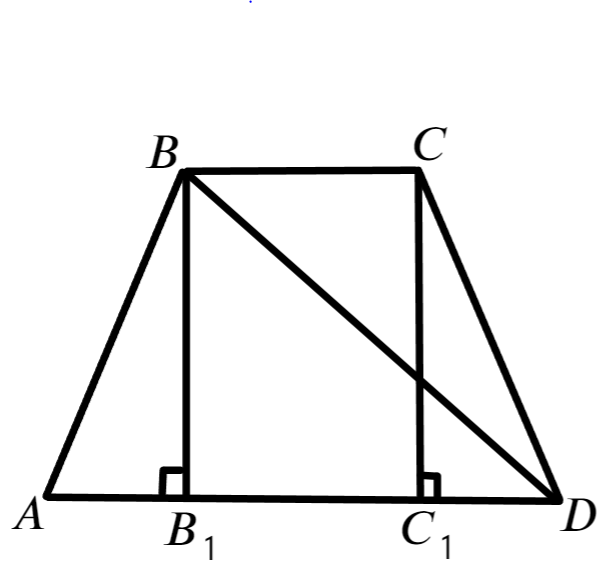
\includegraphics[scale=0.35]{g9-194.png}}
\end{figure}\\
Опустим высоты $BB_1$ и $CC_1,$ тогда $AB_1=C_1D=\cfrac{25-7}{2}=9$ и по теореме Пифагора $BB_1=\sqrt{225-81}=12,\ BD=\sqrt{144+(7+9)^2}=20.$ В треугольнике $ABD$ имеет место соотношение $AB^2+BD^2=225+400=625=AD^2,$ значит по обратной теореме Пифагора он является прямоугольным и центр его описанной окружности --- это середина его гипотенузы $AD.$ Аналогично эта точка является также и центром описанной окружности треугольника $ACD,$ а значит и всей трапеции, ч.т.д.\newpage\noindent
